\documentclass[UTF8, 12pt, a4paper, oneside]{ctexart}
\usepackage{listing}

\usepackage{amsmath}
\usepackage{amsfonts}
\usepackage{geometry}
\usepackage{ulem}
\usepackage[most]{tcolorbox}
\usepackage[hidelinks]{hyperref}
\usepackage{color}
\usepackage{xcolor}
\usepackage{framed}
\usepackage{mathtools,amssymb}
\usepackage{bm}
\usepackage{enumitem}

\definecolor{backcolour}{rgb}{0.18,0.18,0.18}
\definecolor{codegray}{rgb}{0.93,0.93,0.93}
\definecolor{codegreen}{rgb}{0.34,0.76,0.34}
\definecolor{codeblue}{rgb}{0.27,0.35,0.69}
\definecolor{codepurple}{rgb}{0.69,0.25,0.82}
\definecolor{codeorange}{rgb}{0.8,0.6,0.2}
\definecolor{codered}{rgb}{0.8,0.25,0.33}


\lstset{
    backgroundcolor     =   \color{codegray},
    basicstyle          =   \sffamily,          % 基本代码风格
    keywordstyle        =   \bfseries,          % 关键字风格
    commentstyle        =   \rmfamily\itshape,  % 注释的风格,斜体
    stringstyle         =   \ttfamily,  % 字符串风格
    flexiblecolumns,                % 别问为什么,加上这个
    numbers             =   left,   % 行号的位置在左边
    showspaces          =   false,  % 是否显示空格,显示了有点乱,所以不现实了
    numberstyle         =   \zihao{-5}\ttfamily,    % 行号的样式,小五号,tt等宽字体
    showstringspaces    =   false,
    captionpos          =   t,      % 这段代码的名字所呈现的位置,t指的是top上面
    aboveskip           =   1em,
    belowskip           =   1em,
    frame               =   lrtb,   % 显示边框
}

\lstdefinestyle{C++}{
    language        =   C++, % 语言选Python
    basicstyle      =   \zihao{-5}\ttfamily,
    numberstyle     =   \zihao{-5}\ttfamily,
    keywordstyle    =   \color{blue},
    keywordstyle    =   [2] \color{teal},
    stringstyle     =   \color{magenta},
    commentstyle    =   \color{red}\ttfamily,
    breaklines      =   true,   % 自动换行,建议不要写太长的行
    columns         =   fixed,  % 如果不加这一句,字间距就不固定,很丑,必须加
    basewidth       =   0.5em,
}

\lstdefinestyle{C}{
    language        =   C, % 语言选Python
    basicstyle      =   \zihao{-5}\ttfamily,
    numberstyle     =   \zihao{-5}\ttfamily,
    keywordstyle    =   \color{codepurple},
    keywordstyle    =   [2] \color{codegray},
    stringstyle     =   \color{magenta},
    commentstyle    =   \color{codegreen}\ttfamily,
    breaklines      =   true,   % 自动换行,建议不要写太长的行
    columns         =   fixed,  % 如果不加这一句,字间距就不固定,很丑,必须加
    basewidth       =   0.5em,
}

\newlist{choices}{enumerate}{2}
\setlist[choices,1]{
  label = \alph*.,       % 设置标签格式为大写字母后跟括号,例如 A)、B) 等
  leftmargin = *,        % 设置左边距,使其与上层列表对齐
  align = left,          % 设置标签对齐方式为左对齐
  labelwidth = 1.5em,    % 设置标签宽度
  itemsep = 0.5em        % 设置列表项之间的距离
}

\title{\texttt{\bf  数据结构 第一次作业}}
\author{学号:2022212408 姓名:胡宇杭}
\date{\today}

\begin{document}
\maketitle

\section{选择题}
    \begin{enumerate}
        \item 从逻辑上可以把数据结构分为 ( \texttt{\bf  C} ) 两大类
            \begin{choices}
                \item 动态结构、静态结构
                \item 顺序结构、链式结构
                \item 线性结构、非线性结构 
                \item 初等结构、构造型结构
            \end{choices}
        \item 下面关于算法的说法正确的是 ( \texttt{\bf  D} )
            \begin{choices}
                \item 算法的时间复杂度一般与算法的空间复杂度成正比
                \item 解决某问题的算法可能有多种,但肯定采用相同的数据结构
                \item 算法的可行性是指算法的指令不能有二义性
                \item 同一个算法,一般情况下实现语言的级别越高,执行效率越低。
            \end{choices}
        \item 在发生非法操作时,算法能够做出适当处理的特性称为 ( \texttt{\bf  B} )
            \begin{choices}
                \item 正确性
                \item 健壮性
                \item 可读性
                \item 可移植性
            \end{choices}
        \item 在存储数据时,通常不仅要存储各数据元素的值,而且还要存储 ( \texttt{\bf  C })
            \begin{choices}
                \item 数据的处理方法
                \item 数据元素的类型
                \item 数据元素之间的关系
                \item 数据的存储方法
            \end{choices}
        \item 给定 $N×N$ 的二维数组 $A$,则在不改变数组的前提下,查找数组中最大元素的时间复杂度是 ( \texttt{\bf  A })
            \begin{choices}
                \item $O(N^2)$
                \item $O(NlogN)$
                \item $O(N)$
                \item $O(N^2logN)$
            \end{choices}
    \end{enumerate}

\section{判断题}
    \begin{enumerate}
        \item 数据的逻辑结构是指数据的各数据项之间的逻辑关系 $( \ X \ )$
        \item 顺序存储方式的优点是存储密度大,且插入、删除运算效率高 $( \ X \ )$
        \item 数据的逻辑结构说明数据元素之间的次序关系,它依赖于数据的存储结构 $( \ X \ )$
        \item 算法的优劣与描述算法的语言无关,但与所用的计算机性能有关 $( \ X \ )$
        \item 算法必须有输出,但可以没有输入 $( \ \surd \ )$
        \item 若 $f(n)=O(n^2)$,$g(n)=O(n)$ 那么 $f(n)+g(n)=O(n^2)$  $( \ \surd \ )$
        \item 若 $f(n)=O(n^2)$,$g(n)=O(n)那么 f(n)*g(n)=O(n^3)$  $(\ \surd \ )$
    \end{enumerate}

\section{简答题}
    \begin{enumerate}
        \item 分析程序段中带 $\ “\#” \ $ 语句的执行频度,并给出程序段的时间复杂度
            \begin{choices}
                \item 第一小题
                    \lstinputlisting[style = C]{work1_1.c}
                    \par $“\#”$语句在 $while$ 循环的每一次迭代中都会执行一次,因此, $while$ 循环的迭代次数即为该语句的执行频度。下面分析 $while$ 的迭代次数:
                    \par $while$ 循环的结束条件为 $j > n - 1$,而每一次迭代时 $j$ 的值都会增加 $1$,直至达到结束条件。$j$ 的初始值是 $1$,因此 $while$ 循环共迭代 $n - 1$次,因此该语句的执行频度为 $n-1$。
                    \par 算法共执行了 $n - 1$ 次 $while$ 循环,每次循环执行两条语句,所以时间复杂度为 $O(2(n - 1)) = O(n)$。
                \item 第二小题
                    \lstinputlisting[style = C]{work1_2.c}
                    \par 当 $i \leq \frac{n}{2}$ 时, 内层循环每次会执行 $n - 2i + 1$次,当 $i > \frac{n}{2}$ 时,$j$ 的初始值为 $2i > n$,此时不会进行内层循环,故内层循环共进行了 $\sum_{i = 1}^{\frac{n}{2}}(n - 2i + 1) = \frac{n(n-1)}{2}$ 次,即为该语句的执行频度。
                    \par 算法共执行了 $\frac{n^2}{4}$ 次,时间复杂度为 $O(\frac{n^2}{4}) = O(n^2)$。
                \item 第三小题
                    \lstinputlisting[style = C]{work1_3.c}
                    \par 外层循环中, $i$ 从 $0$ 开始递增,共迭代了 $n$ 次,内层循环中 $j$ 从 $i$ 开始递增,共迭代了 $n - i$ 次,故该语句的执行频度为 $\sum_{i = 0}^{n - 1}n - i = \frac{n(n + 1)}{2}$,时间复杂度为 $O(\frac{n(n + 1)}{2}) = O(n^2)$。
                \item 第四小题
                    \lstinputlisting[style = C]{work1_4.c}
                    \par 外层循环中, $i$ 从 $0$ 开始递增,共迭代了 $n$ 次,内层循环中 $j$ 从 $1$ 开始,每次迭代左移一位,即 $j *= 2$,共迭代了 $\lceil log_2n \rceil$ 次,故语句的执行频度为 $n \lceil log_2n \rceil$,时间复杂度为 $O(n \lceil log_2n \rceil) = O(nlog_2n)$。
            \end{choices}
        \item 有的情况下,算法中基本操作重复执行的次数还随问题的输入数据集不同而不同。假定对包含 $1, 2, 3, 4, 5$ 共五个元素的序列 (即 $n = 5$)做冒泡排序,请举例说明何时会出现以下情况:
            \begin{choices}
                \item 任何元素都无需移动
                    \par 当序列为 \texttt{\bf  \ 1, \ 2, \ 3, \ 4, \ 5 \ } 时无需移动。因为对于每一对相邻元素,其顺序都是正确的,无需交换。
                \item 某元素会一度朝着远离预期最终位置的方向移动
                    \par 当序列为 \texttt{\bf  \ 5, \ 4, \ 2, \ 3, \ 1 \ } 时,第一次遍历时会交换 $(5, 4)$,导致 $4$ 向远离预期最终位置的方向移动。
                \item 某元素初始时已位于最终位置,却需要参与 $n - 1$ 次交换
                    \par 当序列为 \texttt{\bf  \ 5, \ 4, \ 3, \ 2, \ 1 \ } 时,所有元素都需要参与 $n - 1$ 次交换,而 $3$ 刚好处于最终位置上。
                \item 所有元素都需要参与 $n - 1$ 次交换
                    \par 序列 \texttt{\bf  \ 5, \ 4, \ 3, \ 2, \ 1 \ }
            \end{choices}
        \item 阅读高质量 $C++/C$ 编程指南或其他 $C$ 编程资料,回答以下问题
            \begin{choices}
                \item 头文件的作用是什么,头文件中为什么有 $ifndef/define/endif$ 结构的预处理块?
                    \par \texttt{\bf 头文件的作用:}
                    \begin{itemize}
                        \item \texttt{\bf 声明和定义:}头文件通常包含函数声明、变量声明、类型定义(如结构和类)以及模板定义。这允许多个源文件共享相同的声明和定义,从而实现代码的模块化和重用;
                        \item \texttt{\bf 代码组织:}头文件提供了一种将代码组织成逻辑单元的方法,使得代码更易于管理和维护;
                        \item \texttt{\bf 参数化编码:}通过宏定义和条件编译,头文件可以用于参数化编码,从而为不同的目标和平台生成不同的代码版本。
                    \end{itemize}
                    \par \texttt{\bf 预处理块的作用:}其目的是防止头文件被多次包含,从而导致重复的声明或定义,进而导致编译错误。
                    \item 引用和指针有何区别?下面代码中的 $Test$ 函数的语句 $GetMemory(str, 200)$ 并没有使 $str$ 获得期望的内存,$str$ 依旧是 $NULL$,请问是为什么,应该如何修改?
                        \lstinputlisting[style = C]{work2_1.c}
                        \par 本质上来说,引用是一个 \texttt{\bf 常量指针} ;从定义上来看,指针是一个变量,其值为另一个变量的地址,其空值可以是 $NULL$,可以在其生命周期中指向不同的对象;引用是另一个已存在变量的别名,一旦初始化,引用就不能再指向其他变量,空值不能为 $NULL$,一旦初始化后,就不能重新绑定到另一个对象。
                        \par \texttt{\bf 原因:}$p$ 是临时变量,在程序中,只是将 $str$ 的值 $(NULL)$ 传给了 $p$,然后为临时变量 $p$ 开辟了内存空间,并不对 $str$ 产生影响。
                        \par \texttt{\bf 修改:}将 $GetMemory()$ 函数中的 $char \ *p$ 改为 $char **p$。
                        \lstinputlisting[style = C, title = {\bf 修改后的程序}]{work2_1_1.c}
                \item 函数体内的局部变量在函数结束时会自动消亡,那么函数体内动态申请的内存是否会自动释放?
                    \lstinputlisting[style = C]{work2_3.c}
                    \par 不会,函数体内的局部变量会存放在栈中,在函数结束时会自动释放内存;而动态申请的内存为堆区内存,需要手动释放。
            \end{choices}
        \item 在调试程序时如果循环在执行 $100$ 次后会出现问题,应如何设置断点进行调试?在调试程序时如果需要在被监控变量的值发生改变时停止执行进行分析,应如何设置?
            \par 以 $Xcode$ 为例进行操作:
            \begin{enumerate}
                \item 先左键点击需要添加断点的位置;
                    \begin{figure*}[h]
                        \centering
                        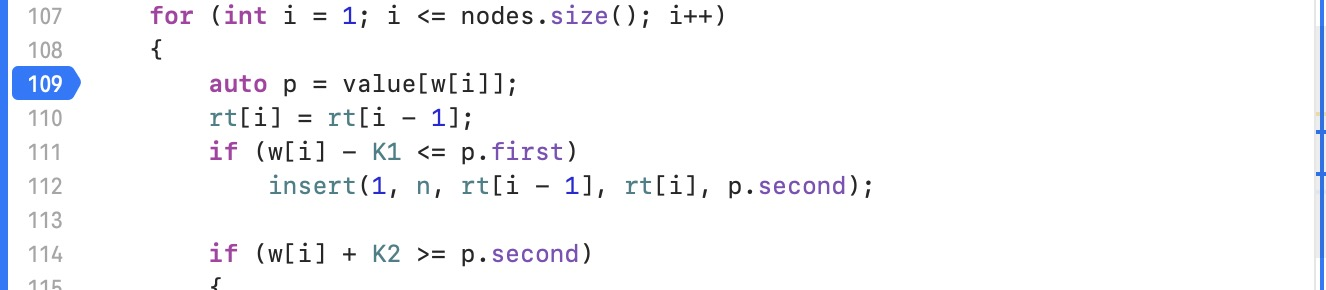
\includegraphics[width=1\textwidth]{step1.jpg}
                    \end{figure*}
                \item 右键断点,选择 \texttt{\bf Edit Breakpoint...};
                    \begin{figure*}[h]
                        \centering
                        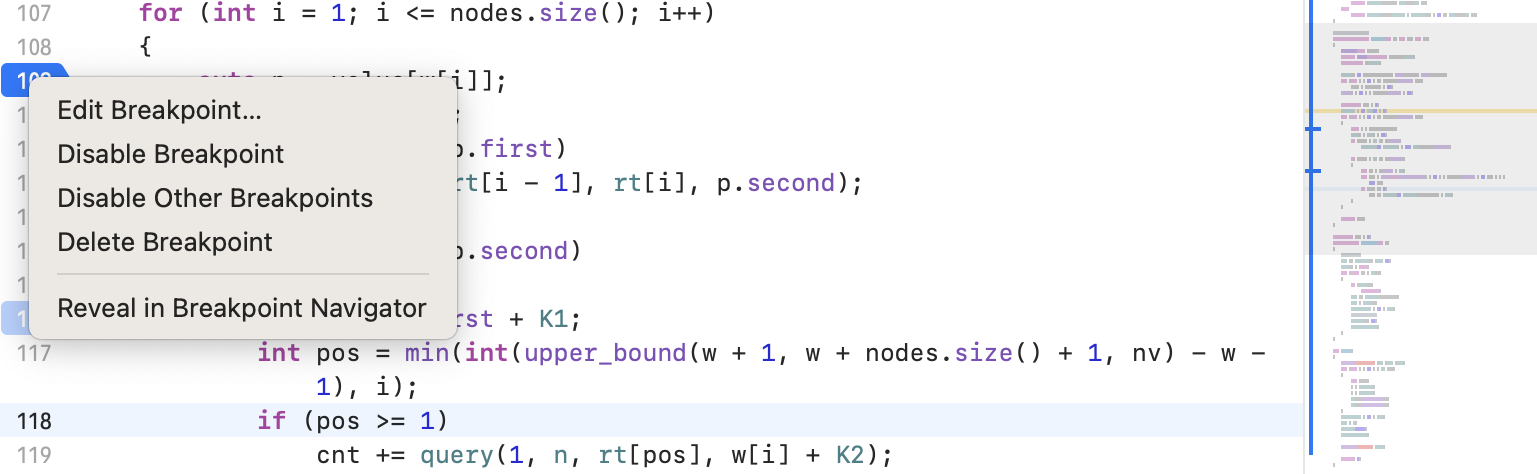
\includegraphics[width=1\textwidth]{step2.png}
                    \end{figure*}
                \item 因为在 $i >= 100$ 时会出现问题,所以在 \texttt{\bf Condition} 中输入 \texttt{\bf i == 99};
                    \begin{figure*}[h]
                        \centering
                        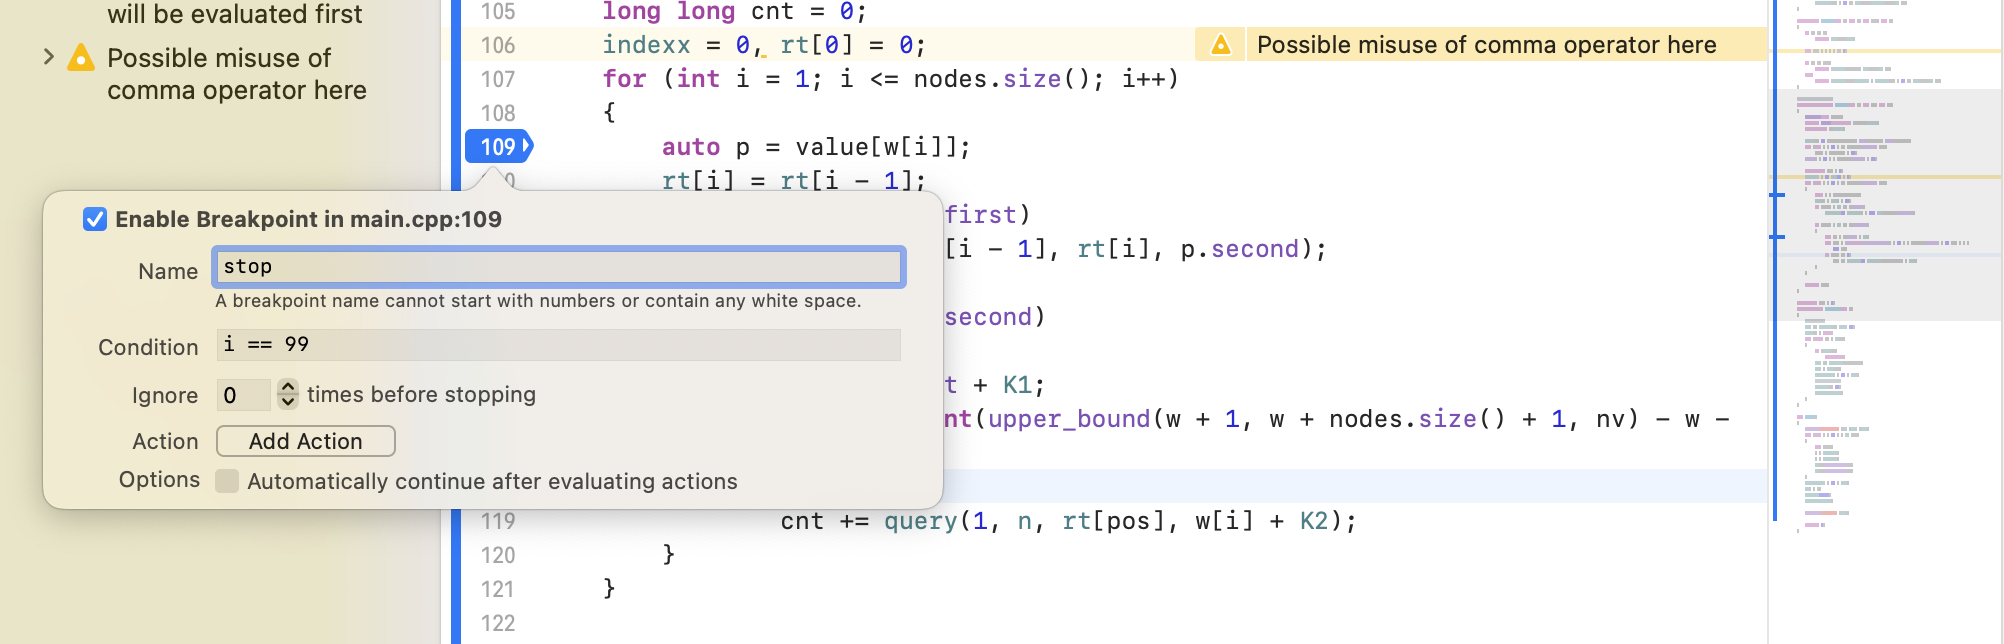
\includegraphics[width=1\textwidth]{step3.png}
                    \end{figure*}
                \item 继续运行程序,发现 \texttt{\bf i == 99} 时程序停止。
                    \begin{figure*}[h]
                        \centering
                        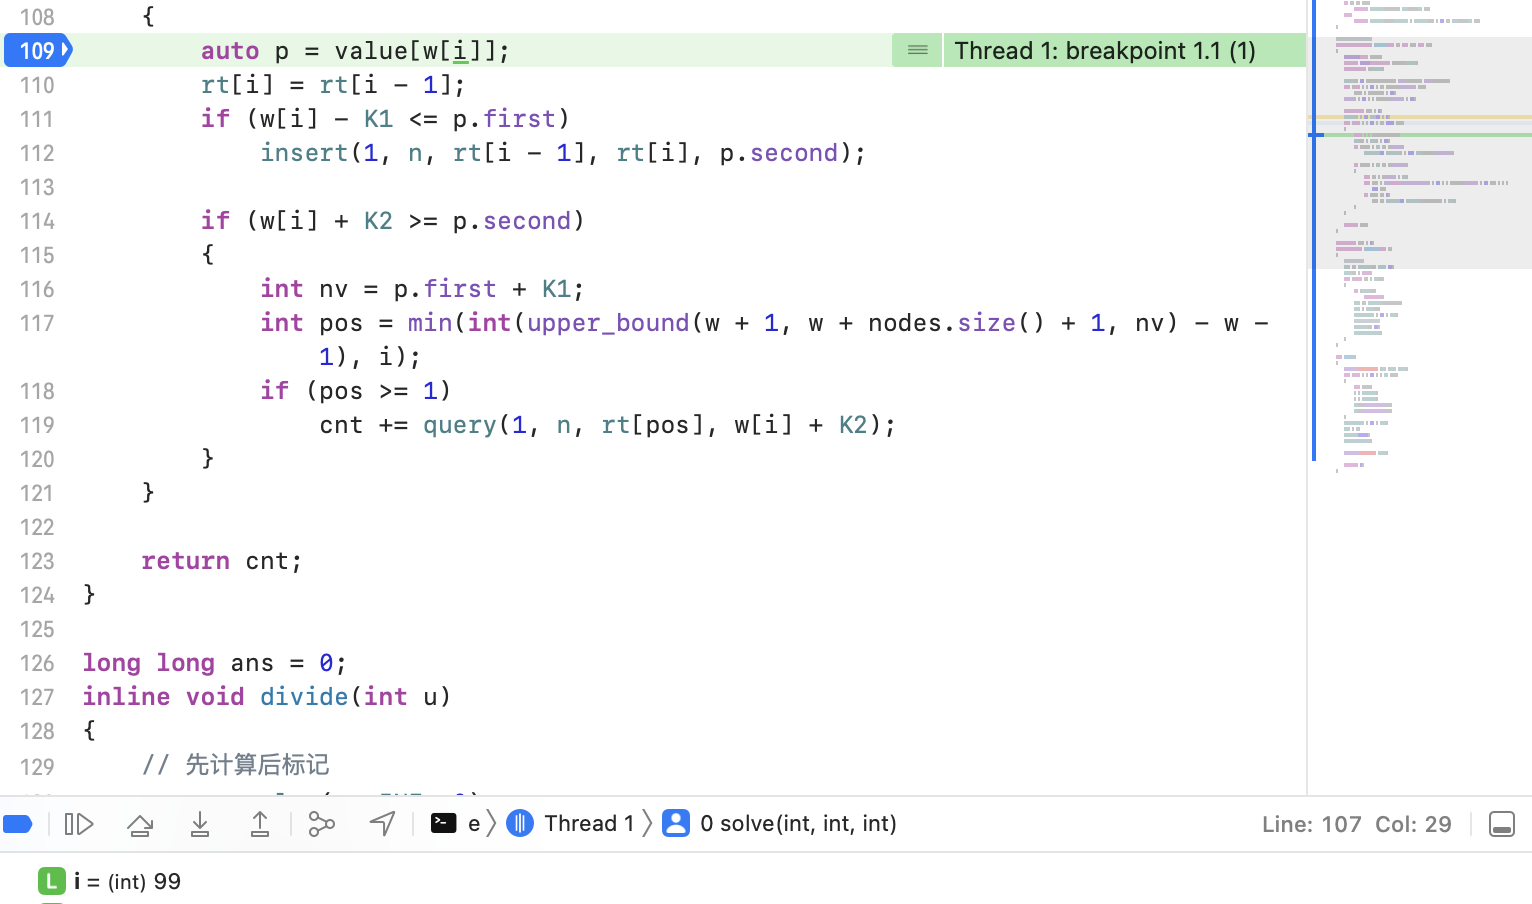
\includegraphics[width=0.9\textwidth]{step4.png}
                    \end{figure*}
                    \newpage
                \item 接下来设置监视,在程序运行时在监视窗口左键点击想要监视的变量;右键,选择 \texttt{\bf Watch ``elem"};
                    \begin{figure*}[h]
                        \centering
                        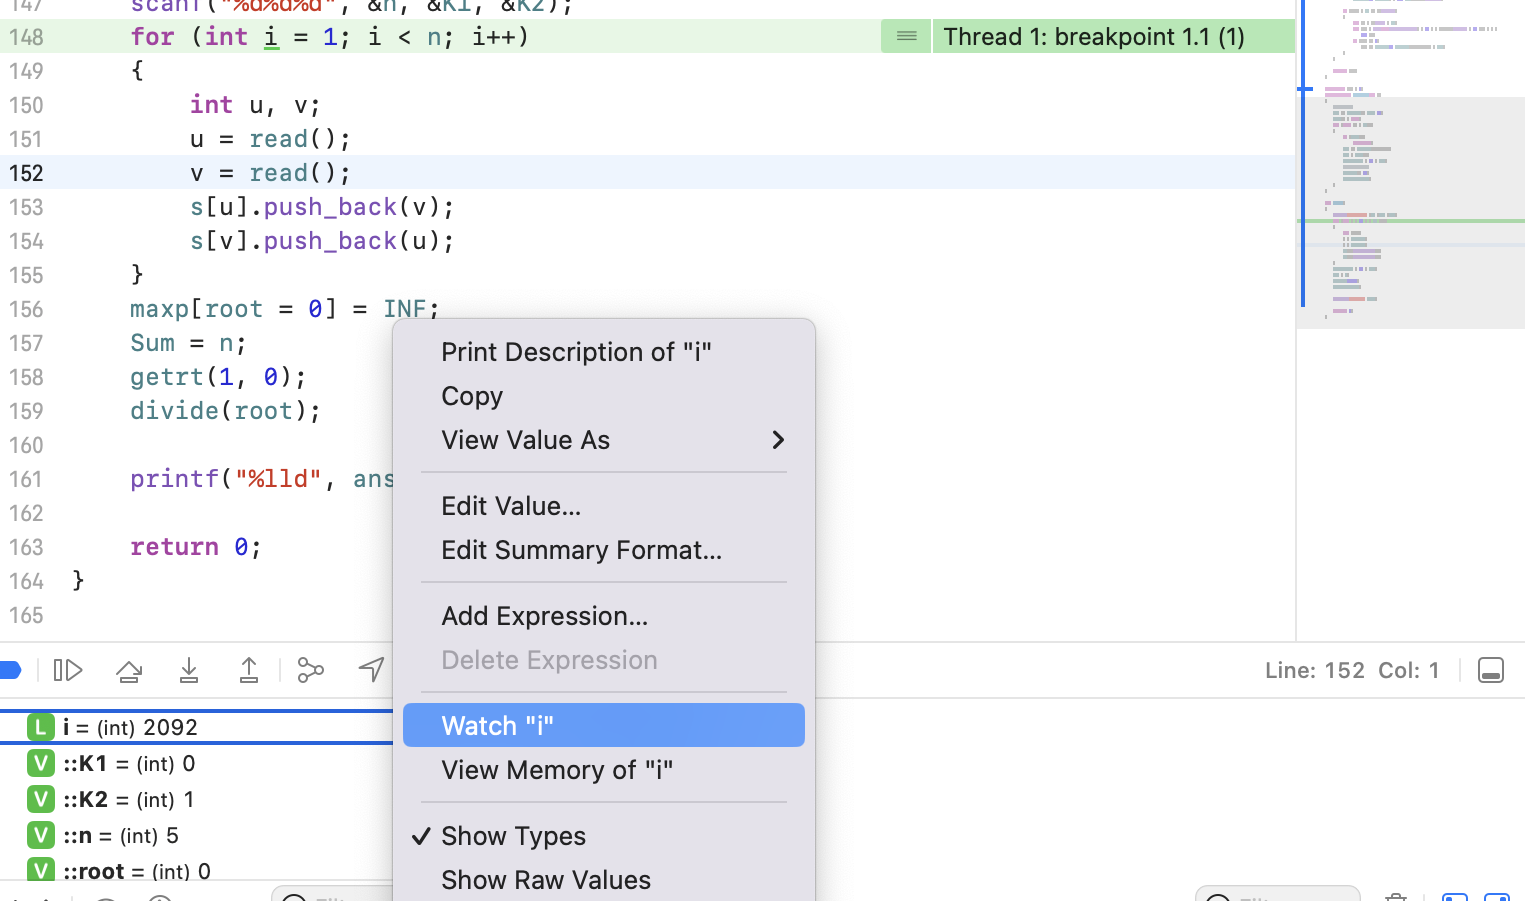
\includegraphics[width=0.85\textwidth]{step5.png}
                    \end{figure*}
                    \newpage
                \item 继续运行,发现在 \texttt{\bf i} 发生变化时程序暂停,并且输出了 \texttt{\bf i} 的变化值。
                    \begin{figure*}[h]
                        \centering
                        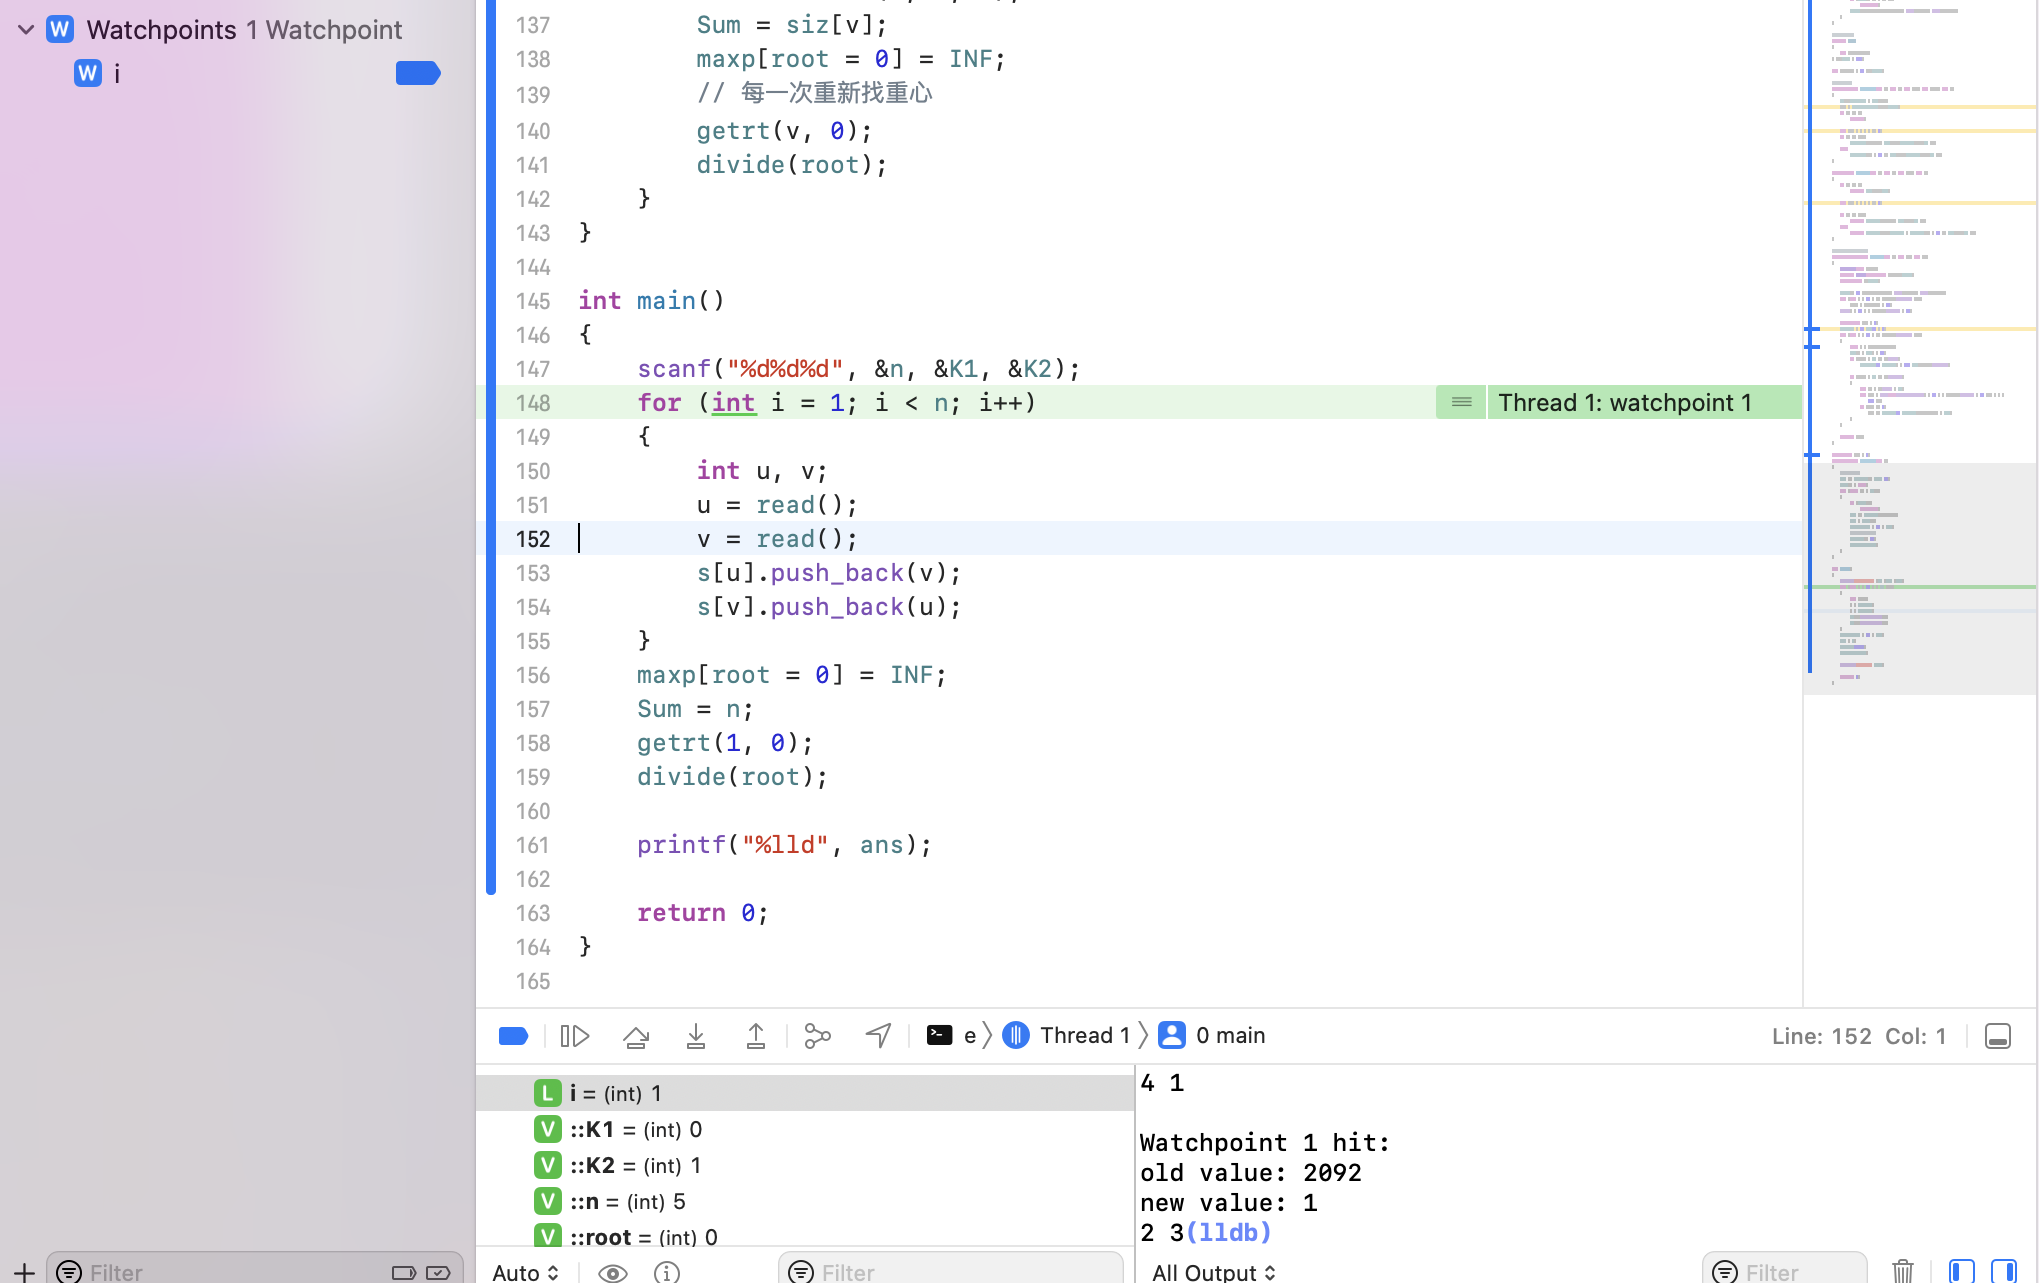
\includegraphics[width=1\textwidth]{step6.png}
                    \end{figure*}
            \end{enumerate}
    \end{enumerate}
\end{document}
            